\documentclass[11pt]{article}
%\usepackage{extsizes}
\usepackage{amsmath, amssymb}
\usepackage{amsthm}
%\usepackage{omegavn,ocmrvn}
%\usepackage[utf8x]{inputenc}
\usepackage[utf8]{vietnam}

\usepackage{longtable}
\usepackage{answers}
\usepackage{graphicx}
\usepackage{array}
\usepackage{pifont}
\usepackage{picinpar}
\usepackage{enumerate}
%\usepackage[top=3.0cm, bottom=3.5cm, left=3.5cm, right=2.5cm] {geometry}
\usepackage{subeqnarray}
\usepackage[backref=page]{hyperref}

\newtheorem{bt}{Câu}
\Newassociation{sol}{Solution}{ans}
\newtheorem{ex}{Câu}
\renewcommand{\solutionstyle}[1]{\textbf{ #1}.}

\newcommand{\reals}{\mathbb{R}}
\newcommand{\complex}{\mathbb{C}}

\def\leq{\leqslant}
\def\rar{\rightarrow}

\def\hro{\mathbb}
\def\R{\hro{R}}
\def\C{\hro{C}}
\def\N{\hro{N}}
\def\Z{\hro{Z}}
\def\bbI{\mathbb{I}}

\def\a{\alpha}
\def\ta{\widetilde{\alpha}}
\def\b{\beta}
\def\de{\delta}
\def\De{\Delta}
\def\tet{\theta}
\def\Tet{\Theta}
\def\dch{\dot{\chi}}
\def\ch{\chi}
\def\ka{\kappa}
\def\vp{\varphi}

\def\dtau{\Delta_{\tau}}
\def\idtau{\Delta_{-\tau}}

\def\ga{\gamma}
\def\Si{\Sigma}
\def\si{\sigma}
\def\om{\omega}
\def\lb{\lambda}
\def\fr{\frac}

\def\tp{\tilde{p}}
\def\tu{\tilde{u}}

\def\frE{\mathfrak{E}}
\def\frA{\mathfrak{A}}
\def\frB{\mathfrak{B}}
\def\frC{\mathfrak{C}}
\def\frD{\mathfrak{D}}
\def\frg{\mathfrak{g}}
\def\frf{\mathfrak{f}}
\def\frX{\mathfrak{X}}
\def\frZ{\mathcal{Z}}

\def\frM{\mathcal{M}}
\def\frP{\mathcal{P}}
\def\frG{\mathfrak{G}}
\def\tfrM{\tilde{\mathcal{M}}}
\def\tfrN{\tilde{\mathcal{N}}}
\def\tfrP{\tilde{\mathcal{P}}}
\def\tfrG{\tilde{\mathcal{G}}}

\def\hfrg{\hat{\mathfrak{g}}}
\def\tfrg{\tilde{\mathfrak{g}}}
\def\hmu{\hat{\mu}}

\def\bbM{\mathbb{M}}
\def\bbN{\mathbb{N}}

\def\hr{\hat{r}}
\def\hv{\hat{v}}
\def\hm{\hat{m}}
\def\hw{\hat{w}}

\def\tP{\tilde{P}}
\def\tQ{\tilde{Q}}
\def\tH{\tilde{H}}
\def\tK{\tilde{K}}

\def\tE{\widetilde{E}}
\def\hE{\hat{E}}
\def\tA{\widetilde{A}}
\def\hA{\hat{A}}
\def\bA{\breve{A}}
\def\tB{\widetilde{B}}
\def\hB{\hat{B}}

\def\hR{\hat{R}}
\def\hS{\hat{S}}
\def\hT{\hat{T}}

\def\tR{\tilde{R}}
\def\tS{\tilde{S}}
\def\tT{\tilde{T}}

\def\tU{\tilde{U}}
\def\tk{\tilde{k}}
\def\hk{\hat{k}}
\def\tX{\tilde{X}}
\def\hX{\hat{X}}
\def\bX{\breve{X}}

\def\tm{\tilde{m}}
\def\bM{\breve{M}}
\def\hM{\hat{M}}
\def\tM{\widetilde{M}}

\def\tmu{\tilde{\mu}}

\def\bE{\breve{E}}
\def\bA{\breve{A}}
\def\bB{\breve{B}}
%\def\uE{\u{E}}
%\def\uA{\u{A}}
%\def\uB{\u{B}}

\def\bbM{\mathbb{M}}
\def\btM{\widetilde{\mathbb{M}}}

\def\hW{\widehat{W}}
\def\tW{\tilde{W}}

\def\hN{\widehat{N}}
\def\tN{\widetilde{N}}

\def\cP{{\cal P}}
\def\cQ{{\cal Q}}
\def\cU{{\cal U}}

\def\cF{{\cal F}}
\def\cG{{\cal G}}
\def\hcF{\hat{\cF}}
\def\hcG{\hat{\cG}}

\def\hcP{\hat{\cP}}
\def\hcQ{\hat{\cQ}}



\def\hS{\widehat{S}}
\def\hZ{\widehat{Z}}
\def\hH{\hat{H}}
\def\hG{\hat{G}}

\def\tx{\tilde{x}}
\def\tf{\tilde{f}}
\def\hf{\hat{f}}
\def\brf{\breve{f}}
\def\brg{\breve{g}}
\def\baf{\bar{f}}
\def\tg{\tilde{g}}
\def\hg{\hat{g}}
\def\ha{\hat{a}}
\def\hd{\hat{d}}
\def\hu{\hat{u}}

\def\cg{\mathcal{g}}
\def\ti{\times}


\def\be{\begin{equation}}
\def\ee{\end{equation}}
\newcommand{\ben}{\begin{eqnarray}}
\newcommand{\een}{\end{eqnarray}}
\newcommand{\bens}{\begin{eqnarray*}}
\newcommand{\eens}{\end{eqnarray*}}
\def\bc{\begin{cases}}
\def\ec{\end{cases}}
\newcommand{\bsq}{\begin{subequations}}
\newcommand{\esq}{\end{subequations}}

\newcommand{\m}[1]{
\begin{bmatrix}
 #1
\end{bmatrix}
}

\renewcommand{\pm}[1]{
\begin{matrix}
 #1
\end{matrix}
}

\newcommand{\doublehat}[1]{%
    \widehat{\widehat{#1\,}}
    }

\newcommand {\mpar}[1]{\marginpar{\fussy\tiny #1}} % marginal notes
\newcommand{\tcal}[1]{%
    \widetilde{\cal{#1}}
    }

    \newcommand{\hcal}[1]{%
    \widehat{\cal{#1}}
    }

    \newcommand{\bcal}[1]{%
    \breve{\cal{#1}}
    }

\newcommand{\bsp}[1]{
\begin{split}
 #1
\end{split}
}
\def\ddt{\fr{\mathrm{d}}{\mathrm{d}t}}

\newcommand{\eproof}{\space
    {\ \vbox{\hrule\hbox{\vrule height1.3ex\hskip0.8ex\vrule}\hrule}}\\[0.2cm]}
    
\def\bce{\begin{compactenum}}
\def\ece{\end{compactenum}}

\newcommand {\corank}   {\mathop{\rm corank}\nolimits}
\newcommand {\range}  {\mathop{\rm range}\nolimits}
\newcommand {\corange}  {\mathop{\rm corange}\nolimits}
\newcommand {\kernel}   {\mathop{\rm kernel}\nolimits}
\newcommand {\cokernel} {\mathop{\rm cokernel}\nolimits}

\begin{document}
% \noindent
\begin{tabular*}
{\linewidth}{c>{\centering\hspace{0pt}} p{.7\textwidth}}
Trường ĐHKHTN, ĐHQGHN & {\bf Học Kỳ 2 (2020-2021)}
\tabularnewline
K63 CNKHTN & Mã môn học: MAT3342
\tabularnewline
\rule{1in}{1pt}  \small  & \rule{2in}{1pt} %(Due date:)
\tabularnewline

%  \tabularnewline
%  &(Đề thi có 1 trang)
\end{tabular*}
%
% \Opensolutionfile{ans}[ans1]

\begin{center}
Bài tập lớn: Lý thuyết hệ điều khiển tuyến tính \\ Thời hạn nộp bài: 09/05/2021
\end{center}

\begin{bt}
	Một hệ điều khiển tuyến tính bậc 2 có dạng 
	\begin{align}\label{eq1}
		& M \ddot{x}(t) + K x(t) = B u(t), \mbox{ với mọi } t\geq 0, \quad \dot{x}(0)=\dot{x}_0, \ x(0) = x_0, \\  
		& y = C x(t) + \tilde{D} u(t),
	\end{align}
	trong đó $M$, $K \in \R^{n,n}$ là các ma trận giá trị thực thể hiện trọng và độ cứng; $M$ là khả nghịch, $x(t)\in \R^n$, $B\in \R^{n,p}$, $u(t) \in \R^p$, $C \in \R^{q,n}$, $\tilde{D}\in \R^{q,p}$. Ta gọi $M$, $K$, $B$, $C$, $\tilde{D}$ là các ma trận hệ số của hệ.
	\begin{enumerate}
		\item[i)] Hệ \eqref{eq1} được gọi là \emph{dương trong (internally positive)} nếu như với mọi biến điều khiển không âm (tức là $u(t) \geq 0$ với mọi $t\geq 0$) và mọi điều kiện ban đầu không âm (tức là $x_0\geq 0$, $\dot{x}_0\geq 0$) thì trạng thái $x(t)$ và đầu ra $y(t)$ đều không âm.
		\item[ii)] Hệ được gọi là \emph{dương ngoài (externally positive)} nếu trong phần i) ở trên ta chỉ yêu cầu $y(t)\geq 0$ chứ không yêu cầu $x(t) \geq 0$.
	\end{enumerate}
	Đề đơn giản xét trường hợp $M=I_n$ là ma trận đơn vị. \\
	a) Hãy tìm một điều kiện đủ của các ma trận hệ số của hệ \eqref{eq1} để hệ là dương trong. Điều kiện đó có phải là điều kiện cần không? \\
	b) Tìm điều kiện cần và đủ của các ma trận hệ số của hệ \eqref{eq1} để hệ là dương trong. \\
	c) Hãy chỉ ra 1 ví dụ mà hệ là dương ngoài nhưng không là dương trong. \\
	% d) Tìm điều kiện cần và đủ của các ma trận hệ số của hệ \eqref{eq1} để hệ là dương ngoài.
\end{bt}

%\baituluan{GT:2}{ Positive realization of 2nd order descriptor systems: not easy with the new positivity concept.
%\end{bt}
%%Hết câu hỏi 2%

\begin{bt}
	Xét hệ dương bậc nhất dạng
	%
	\begin{align}\label{eq2}
		\dot{x}(t) &= A x(t) + B u(t), \mbox{ với mọi } t \geq 0, \quad x(0)=x_0, \\
		y(t) &= Cx(t),
	\end{align}
	%
	trong đó $A$, $B$, $C$ là các ma trận hệ số. Trong thực tế người ta quan tâm đến các hệ dương và ổn định theo nghĩa sau. % (xem \cite[Chương 5]{Far00}). 
	%
	\begin{enumerate}
		\item[i)] Xét $u \equiv 0$. Khi đó hệ \eqref{eq2} được gọi là \emph{ổn định theo nghĩa Lyapunov} nếu với mọi $\epsilon > 0$ tồn tại $\delta >0$ đủ bé và $N$ đủ lớn sao cho với mọi điều kiện đầu thỏa mãn $\|x_0\|_2 \leq \delta$ thì $\|x(t)\|<\epsilon$ với mọi $t \geq N$. Thêm vào đó, nếu $\lim_{t\rightarrow \infty} x(t) = 0 $ thì ta nói hệ là ổn định tiệm cận. 
		\item[ii)] Hệ \eqref{eq2} được gọi là \emph{ổn định BIBO} nếu với mọi đầu vào $u$ bị chặn đều theo $t$ thì đầu ra $y$ cũng bị chặn đều theo $t$.
	\end{enumerate}
	%
	a) Cho $C \geq 0$. Hãy chứng minh rằng một hệ dương trong bất kỳ dạng \eqref{eq2} là ổn định tiệm cận khi và chỉ khi mọi hệ số của đa thức đặc trưng $\det(\lambda I-A)$ là dương. \\
	b) Cho $C \geq 0$. Hãy chứng minh rằng một hệ dương trong bất kỳ dạng \eqref{eq2} là ổn định tiệm cận khi và chỉ khi mọi định thức con góc trái của $-A$ là dương. \\
	c) Nếu hệ là ổn định tiệm cận hãy chứng minh nó là ổn định BIBO. Điều ngược lại có đúng không? Vì sao?
	%\begin{thebibliography}{9}
	%	\bibitem{Far00} Lorenzo Farina, Sergio Rinaldi, \emph{Positive Linear Systems: Theory and Applications}, John Wiley \& Sons, 2000.
	%\end{thebibliography}	
\end{bt}


\begin{bt}
	a) Hãy xem xét một hệ thống có phản hồi xung như Hình \ref{fig:fig1} (a). Tìm phản hồi trạng thái 0 được kích thích bởi đầu vào u (t) được thể hiện trong Hình (b).
	% TODO: \usepackage{graphicx} required
	\begin{figure}[h!]
		\centering
		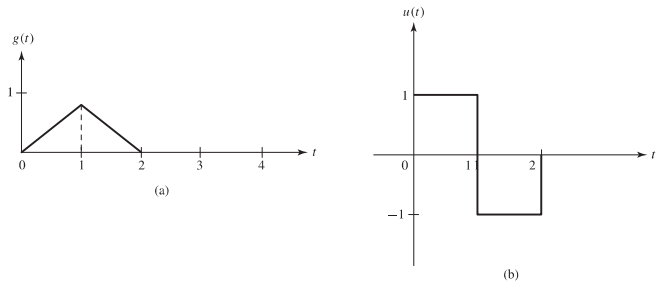
\includegraphics[width=1.0\linewidth]{Fig2.20}
	    \caption{}
		\label{fig:fig1}
	\end{figure}
	%
	
	\noindent b) Xét một hệ 2 đầu vào và 2 đầu ra được biểu diễn bởi phương trình
	\begin{align*}
		& D_{11}(p)y_1(t) + D_{12}(p)y_2(t) = N_{11}(p)u_1(t) + N_{12}(p)u_2(t), \\
		& D_{21}(p)y_1(t) + D_{22}(p)y_2(t) = N_{21}(p)u_1(t) + N_{22}(p)u_2(t)
	\end{align*}
	trong đó $N_{ij}$ and $D_{ij}$ là các đa thức của $p := d/dt$. Tìm ma trận hàm truyền của hệ.\\
	c) Hãy xem xét các hệ thống phản hồi dương và âm được thể hiện trong Hình \ref{fig:fig2} (a) và (b). 
	% TODO: \usepackage{graphicx} required
	\begin{figure}[h!]
		\centering
		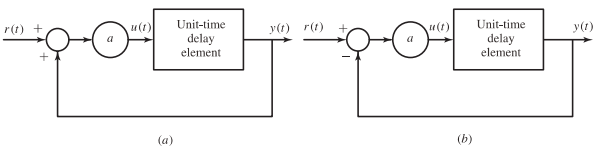
\includegraphics[width=1.0\linewidth]{Fig2.5}
		\caption{Hệ thống điều khiển phản hồi dương và âm}
		\label{fig:fig2}
	\end{figure}
	%
	Chứng tỏ rằng các phản hồi theo bước đơn vị của hệ thống phản hồi dương được thể hiện trong Hình \ref{fig:fig3} (a) cho a = 1 và trong Hình \ref{fig:fig3} (b) cho a = 0.5. Cũng chứng tỏ rằng các phản hồi theo bước đơn vị của hệ thống phản hồi âm được thể hiện trong (c) và (d) tương ứng với a = 1 và a = 0.5.
	%
	% TODO: \usepackage{graphicx} required
	\begin{figure}[h!]
		\centering
		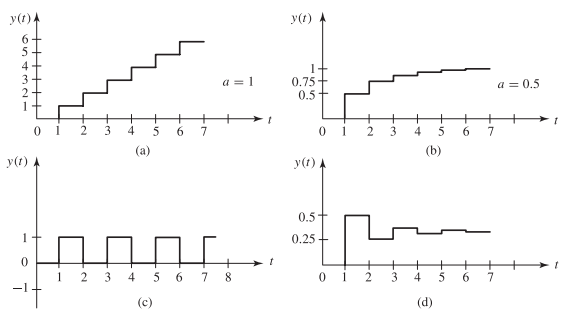
\includegraphics[width=1.0\linewidth]{Fig2.21}
		\caption{}
		\label{fig:fig3}
	\end{figure}
\centerline{——————————— Hết Bài Giữa Kỳ ——————————-}
\pagebreak 
\begin{center}
\textbf{ADDITIONAL EXERCISE FOR THE FINAL EXAM}
\end{center}
\end{bt}

\begin{bt}
a) Resolve the necessary and sufficient condition for the matrix $K\in \R^{n,n}$ such that
\begin{equation*}
\sum_{m\geq 0}\dfrac{1}{(2m)!} (-K)^m t^{2m} \geq 0, \mbox{ and }
\ 
\sum_{m\geq 0}\dfrac{1}{(2m+1)!} (-K)^m t^{2m+1} \geq 0,
\end{equation*}
%
in two cases: i) $K$ is a scalar, and ii) $K$ is a square, symmetric positive definite matrix. \\
b) Solve the general problem for symmetric system (which usually occurs in mechanics), i.e., find the necessary and sufficient condition for the system coefficients in order to verify the internal positivity
%
\[
M \ddot{x}(t) + D \dot{x}(t) + K x(t) = B u(t), \mbox{ for all } t\geq 0,
\]
where the matrices $M$, $K$ are symmetric, positive definite, and $D$ is symmetric, positive semi-definite.
%
\end{bt}

\begin{bt}
Find the necessary and sufficient condition for the matrices M,D,K,B such that the second order system
%
\begin{equation}\label{1}
M \ddot{x}(t) + D \dot{x}(t) + K x(t) = B u(t), \mbox{ for all } t\geq 0,
\end{equation}
%
where $M \in \R^{n,n}$ is invertible, \\
%
a) is $C$-controllable, i.e., for any initial condition $x(0) = x_0$ and $\dot{x}(0) = \dot{x}_0$, and any final state $x_1$, there exists an input that transfers $(x_0,\dot{x}_0)$ to $x_1$ in a finite time. \\
b) is $C_2$-controllable, i.e., transfer from any pair $(x_0,\dot{x}_0) \in \R^{n} \times \R^n$ to any pair $(x_1,\dot{x}_1) \in \R^{n} \times \R^n$. \\
c) is $C$-observable, i.e., for any unknown initial condition $x(0) = x_0$ and $\dot{x}(0) = \dot{x}_0$, there exists a finite time $t_1$ such that 
the pair $(x_0,\dot{x}_0)$ is uniquely determined from the knowledge of 
the input $u|_{[t_0,t_1]}$ and the output $y|_{[t_0,t_1]}$. \
You may think about the equivalent condition, that knowing $y=0$, $u=0$ implies that $(x_0,\dot{x}_0)=(0,0)$.\\
d) Establish and prove the duality of $C$-observability and $C2$-controllability for the original system \eqref{1} and the dual system
%
\begin{equation}\label{2}
M^T \ddot{x}(t) + D^T \dot{x}(t) + K^T x(t) = C^T u(t), \mbox{ for all } t\geq 0 \ .
\end{equation}
%
%
\end{bt}

\begin{bt}
Programming your conditions for the two exercise above in MATLAB/OCTAVE.\\
\verb|function value = check_positive(M,D,K,B)| \\
\verb|function value = check_Cctrb(M,D,K,B)| \\
\verb|function value = check_C2ctrb(M,D,K,B)| \\
\verb|function value = check_Cobsv(M,D,K,B)|
\end{bt}

\vskip 1cm
\centerline{———————————  THE END ——————————-}

\end{document}

\vspace{1cm}
\noindent{\bf Chú ý:} {\it Cán bộ coi thi không giải thích gì thêm}\\
\Closesolutionfile{ans}
\newpage
\begin{center}
{\LARGE{\bf ĐÁP ÁN}}
\end{center}

\begin{sol}
\end{sol}

   
\end{document}



